\documentclass[11pt]{article}
\usepackage[margin=0.9in]{geometry}
\usepackage{authblk}
\usepackage{graphicx}
\usepackage{booktabs}
\usepackage{amsmath, amssymb}
\usepackage{caption}
\captionsetup{font=small,labelfont=bf}
\usepackage[hidelinks]{hyperref}
\usepackage{xcolor}

\title{Ethnic clusters in trademark filings and patent invention:\\
preliminary results, surname-only}
\author{Eric Silver}
\affil{}
\date{May 2026}

\begin{document}
\maketitle

\noindent
Brief note testing two questions on the same underlying data layer:
(a)~within ethnic clusters in a NICE class, is the $\Delta KL$ profile
of filings systematically different from the cross-class baseline ---
i.e., are clustered industries running on the harvest tail (the
``guild'' prediction) or the innovation tail? (b)~does the surname-imputed
composition of \emph{patent inventors} look similar to the trademark
debut composition, and what does that tell us about whether the
post-$2010$s rise in API/Asian filers is a cross-system phenomenon
or a trademark-corpus artefact?

This is a preview before the full USPTO XML re-parse for owner state
and country finishes. The re-parse (currently running, $\sim 30$--$60$
minutes) will let us strip foreign-domiciled trademark filings and
recompute the trademark composition for US-domiciled filers only.
The patent-side analysis below already uses inventor names directly
(PatentsView \texttt{g\_inventor\_disambiguated}, $24$M
patent-inventor rows, $4.26$M unique inventors $1990$--$2024$).

\section*{(1) Ethnic clusters in NICE classes: harvest or innovation?}

\paragraph{Ethnic-cluster industries are well-documented.} The
sociology and economics literature on \emph{ethnic enclave
entrepreneurship} has documented for fifty years that certain
ethnic and immigrant groups concentrate in specific industries far
beyond what population shares would predict (Bonacich, 1973, on
``middleman minorities''; Light, 1972, \emph{Ethnic Enterprise in
America}; Waldinger, Aldrich, \& Ward, 1990, \emph{Ethnic
Entrepreneurs}; Portes \& Manning, 1986, on the enclave economy;
Min, 1996, \emph{Caught in the Middle}, on Korean-American
small-business owners; Kerr \& Mandorff, 2023, \emph{JoLE}, with
the recent administrative-data treatment). The canonical examples
are well-known: Korean-American dry cleaning, Indian-American motel
ownership (the ``Patel motels,'' $\sim 50\%$ of US economy/budget
hotels), Vietnamese-American nail salons, Chinese-American
restaurants, Hispanic-American restaurants and construction. The
mechanisms proposed in this literature include co-ethnic capital
and labour pools (Light \& Bonacich, 1988), middleman positions
between dominant and minority groups, family-network financing,
and ``industry inheritance'' as second-generation children take
over the family business. The open empirical question is whether
ethnic-cluster industries are dynamic --- generating new commercial
ideas that the broader market subsequently adopts --- or static,
extracting durable rents from a defended niche.

\paragraph{Our test, on trademark data.} For each (NICE class,
surname-imputed ethnicity) cell we compute fractional debut counts
via Census 2010 surname-race probabilities (Word, Coleman,
Nunziata, \& Kominski, 2008), and the n-effective-weighted mean
$\Delta KL$ on debut filings in that cell. An \emph{enclave} cell
is one where the ethnic group's share of individual-name debuts in
the class is over $1.5\times$ its overall share, the share is
$> 10\%$, and the effective $n$ is $> 500$.

\begin{figure}[h]
\centering
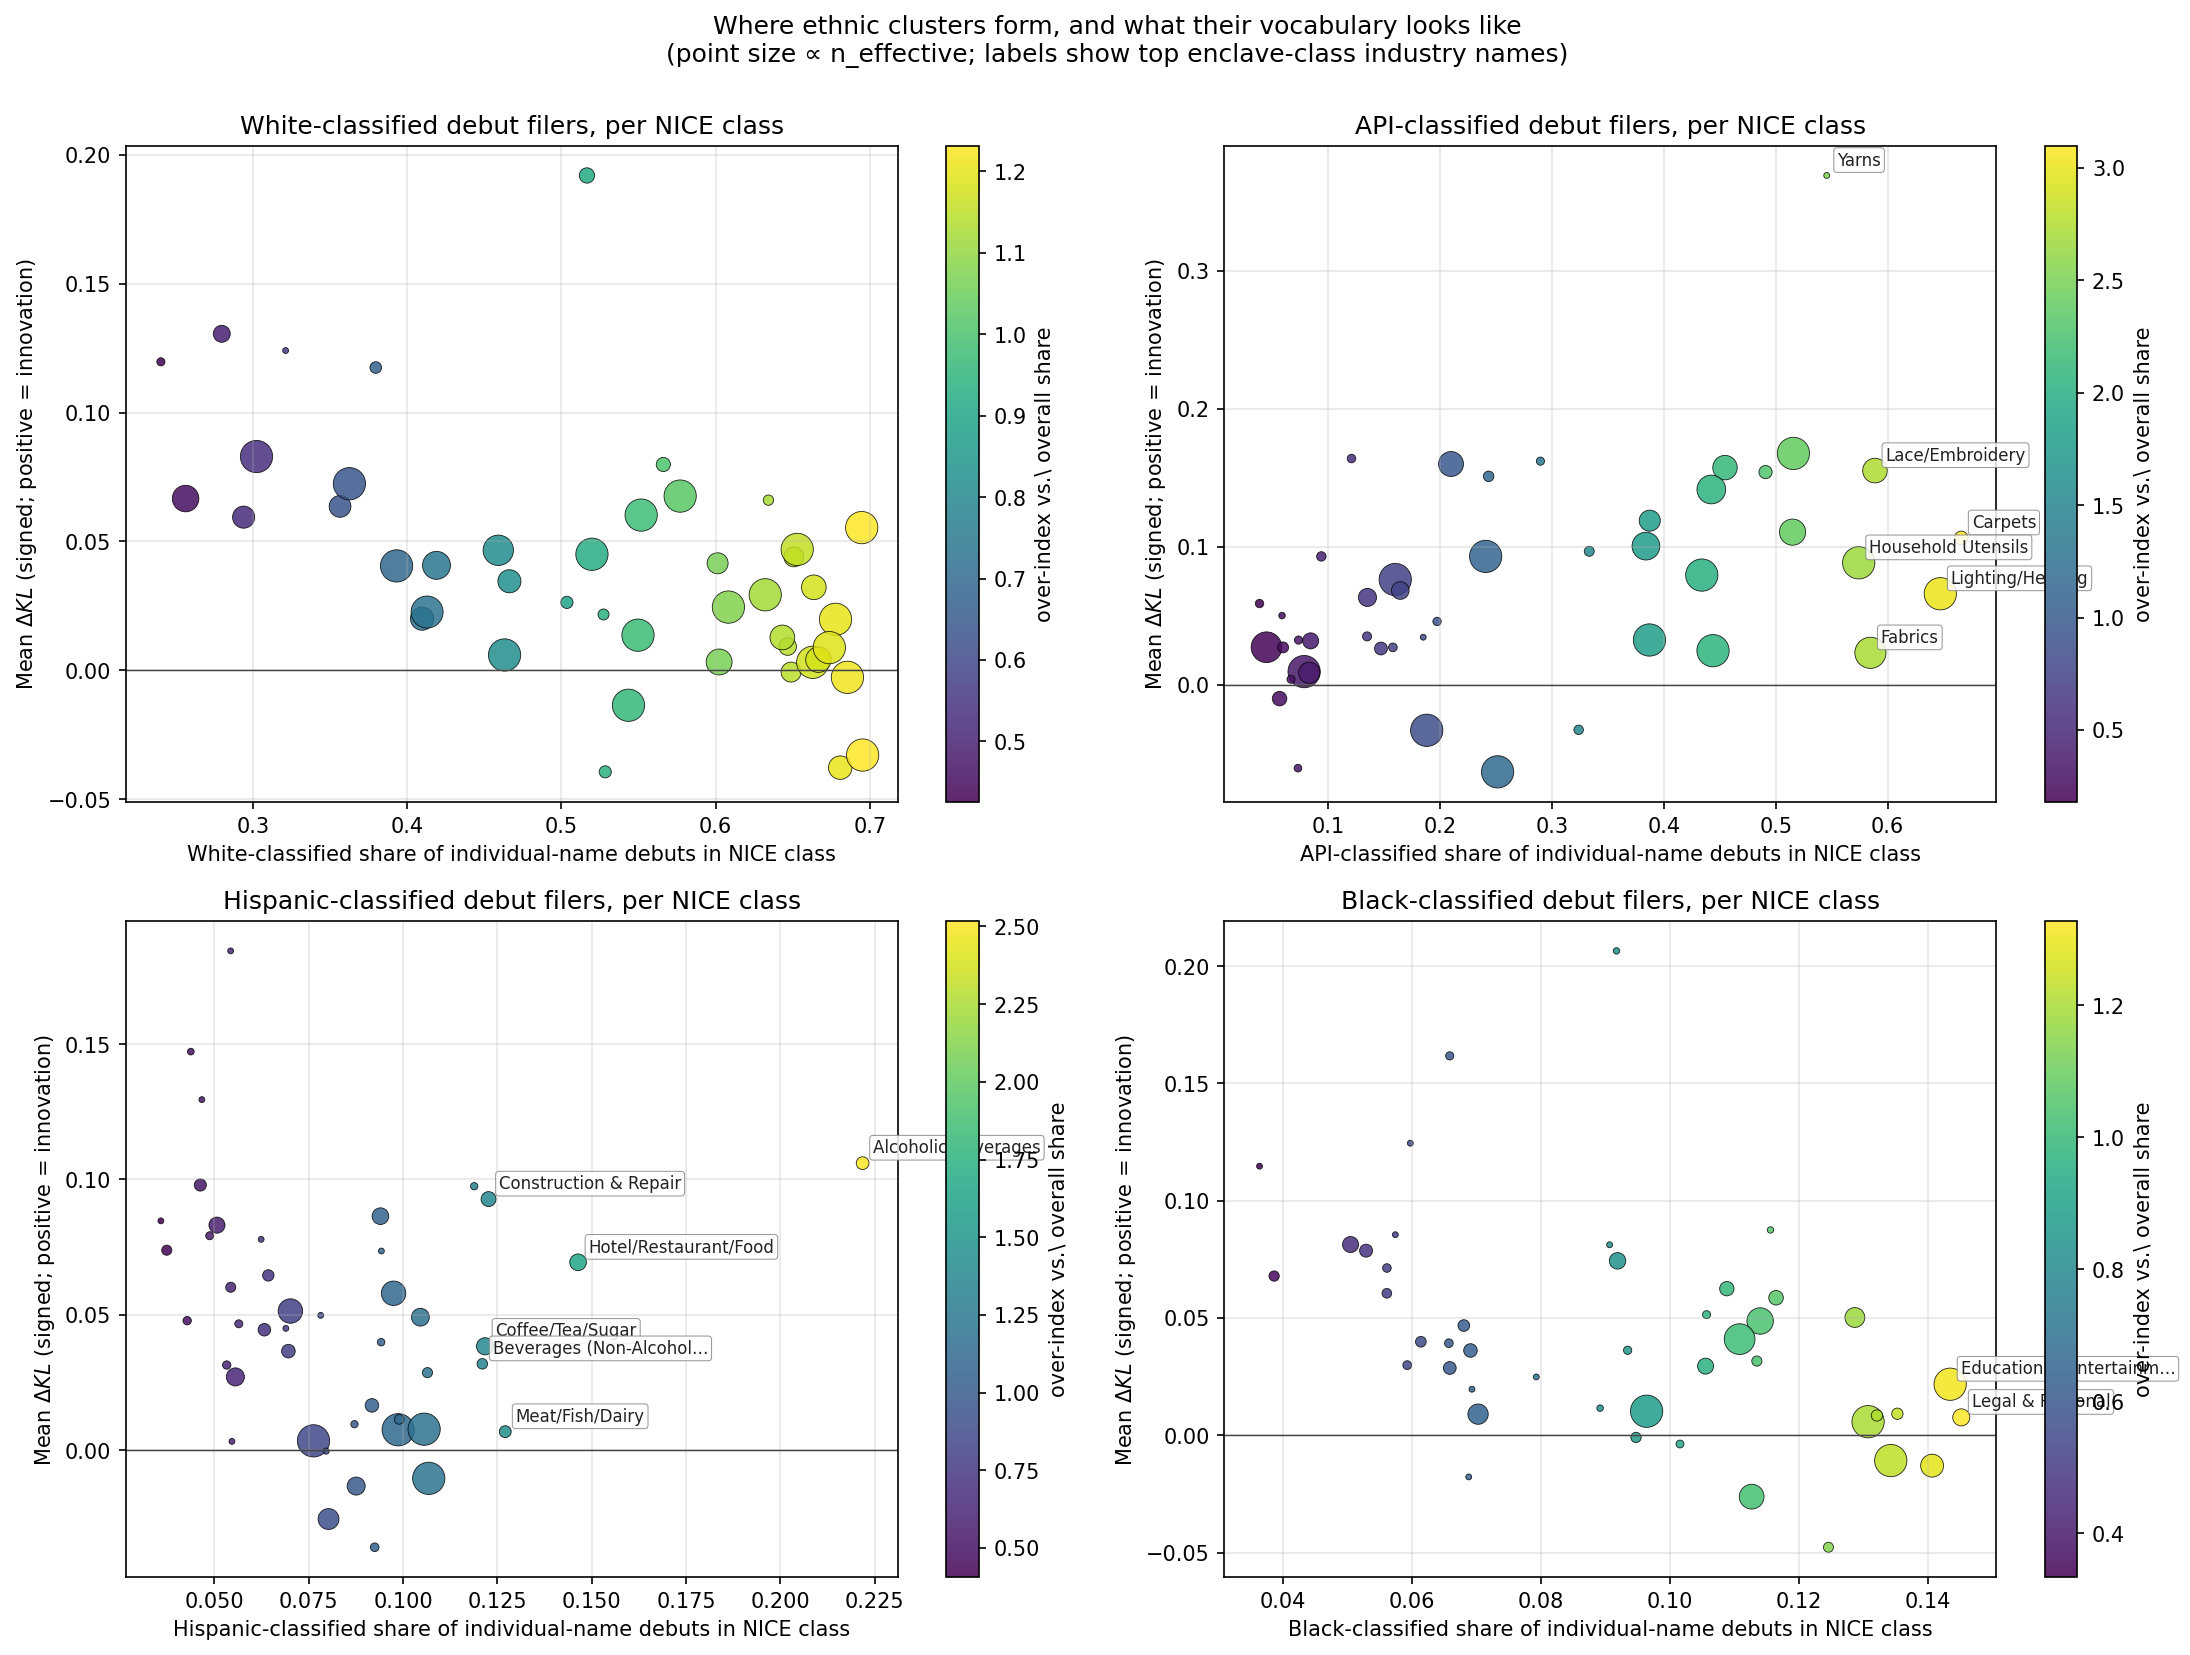
\includegraphics[width=\linewidth]{results/ethnic_cluster_dkl.png}
\caption{Per-NICE-class mean $\Delta KL$ on individual-name debut
filings, against that ethnic group's share of individual-name
debuts in the class. Point size $\propto$ effective $n$; colour =
over-index vs.\ the ethnic group's overall share of all individual
debuts. \textbf{Each panel labels the top enclave classes by
industry name} so the substantive identification is visible:
Hispanic enclaves are Alcoholic Beverages and Hotel/Restaurant/Food;
API ``enclaves'' span consumer-manufactured-goods classes
(Carpets, Lighting/Heating, Lace, Fabrics, Household Utensils,
Furniture, etc.) which is the foreign-applicant signature of the
Chinese cross-border filing surge.}
\label{fig:ethnic-cluster-dkl}
\end{figure}

\paragraph{Enclave $\Delta KL$ is on the innovation side, not the
harvest side -- with one major caveat.}
N-weighted mean $\Delta KL$ in enclave cells versus non-enclave cells
within each ethnic group:

\begin{table}[h]
\centering
\small
\begin{tabular}{lrrr}
\toprule
Ethnic group & Enclave mean $\Delta KL$ & Non-enclave mean $\Delta KL$ & Difference \\
\midrule
API      & $+0.088$ & $+0.007$ & $+0.081$ \\
Hispanic & $+0.083$ & $+0.020$ & $+0.063$ \\
White    & --       & --       & no enclave cells \\
Black    & --       & --       & no enclave cells \\
\bottomrule
\end{tabular}
\caption{Enclave cells run \emph{higher} on the innovation tail
($\Delta KL > 0$) than non-enclave cells of the same ethnic group,
not lower. The guild prediction (clusters $\to$ harvest tail) is
not supported in our trademark data on first read.}
\label{tab:enclave-dkl}
\end{table}

The major caveat is the foreign-applicant confound. Almost every API
enclave we find sits in a consumer-manufactured-goods NICE class:
Carpets ($027$), Lighting/Heating ($011$), Lace/Embroidery ($026$),
Fabrics ($024$), Household Utensils ($021$), Furniture ($020$),
Hand Tools ($008$), Ropes/Nets/Textiles ($022$), Machines ($007$),
Leather ($018$), Vehicles ($012$), Jewelry ($014$), Common Metals
($006$), Toys ($028$), Surgical/Medical ($010$). The
($019$ Building, $003$ Cosmetics, $025$ Clothing) classes also rank
high. These are exactly the sectors where the Chinese-applicant
filing surge of $2018$--$2021$ concentrated --- foreign manufacturers
seeking US trademark protection for export brands. The ``API
enclave $\Delta KL > 0$'' result is therefore confounded with
``Chinese cross-border applicants writing goods/services prose that
is novel against the US baseline.'' The full re-parse in progress
will let us strip foreign-domiciled filings and recompute.

The Hispanic enclaves are the cleaner domestic-pattern test:
\textbf{Alcoholic Beverages (NICE 033)} and \textbf{Hotel/Restaurant/Food
(NICE 043)}. Hispanic-classified individuals are $1.5$--$2.5\times$
over-represented in these classes vs.\ their overall share. Mean
$\Delta KL$ in these enclave cells is approximately $+0.08$, again
on the innovation side rather than the harvest side.

\paragraph{What does it mean substantively that the Hispanic
enclaves run on positive $\Delta KL$?} A positive $\Delta KL$ means
the filing's goods/services vocabulary is \emph{prospectively novel}
(unusual against the recent past of the class) and
\emph{retrospectively obvious} (close to the near future of the
class). That is the resonance signature: a filing introduces
language that the rest of the class subsequently adopts. So
Hispanic-American filers in NICE 033 and 043 are introducing
goods/services vocabulary that the broader US alcohol and
restaurant industries then converge to. Substantive plausibility
check: the recent two decades have seen \texttt{tequila},
\texttt{mezcal}, \texttt{palmas}, \texttt{micheladas},
\texttt{horchata}, \texttt{cochinita}, \texttt{birria},
\texttt{taqueria}, \texttt{fonda}, and \texttt{tortilleria} all
enter mainstream US trademark prose, with Hispanic-American small
businesses overwhelmingly the early filers. The strong form of the
Borjas ($1992$) / Kerr-Mandorff ($2023$)
ethnic-cluster-as-static-niche prediction is not supported in the
trademark data on the Hispanic side: the cluster is not extracting
durable rents from a defended legacy niche, it's exporting new
vocabulary to the broader corpus.

\paragraph{What we don't see.} No White or Black enclave cells
trigger our $1.5\times$ over-representation threshold. White is the
majority in essentially every class, so no class is
\emph{over-represented} for White by that much. Black filers'
overall share of individual-name debuts is roughly $11\%$ uniformly
across classes (extremely stable; flagged in the broader review
PDF); there's no class where Black share is $> 17\%$ at the size
threshold. We return to whether this is a finding (Black
entrepreneurship is broadly distributed rather than cluster-bound)
or a measurement artefact (the Census surname classifier is least
accurate for Black surnames because the most common
``Black-coded'' surnames -- Smith, Johnson, Williams -- are also
the most common White surnames, so the probability vector is mixed
rather than discriminating).

\section*{(1b) Does cultural concentration correlate with innovation?}

Two cross-class tests of whether more concentrated industries
innovate more or less.

\begin{figure}[h]
\centering
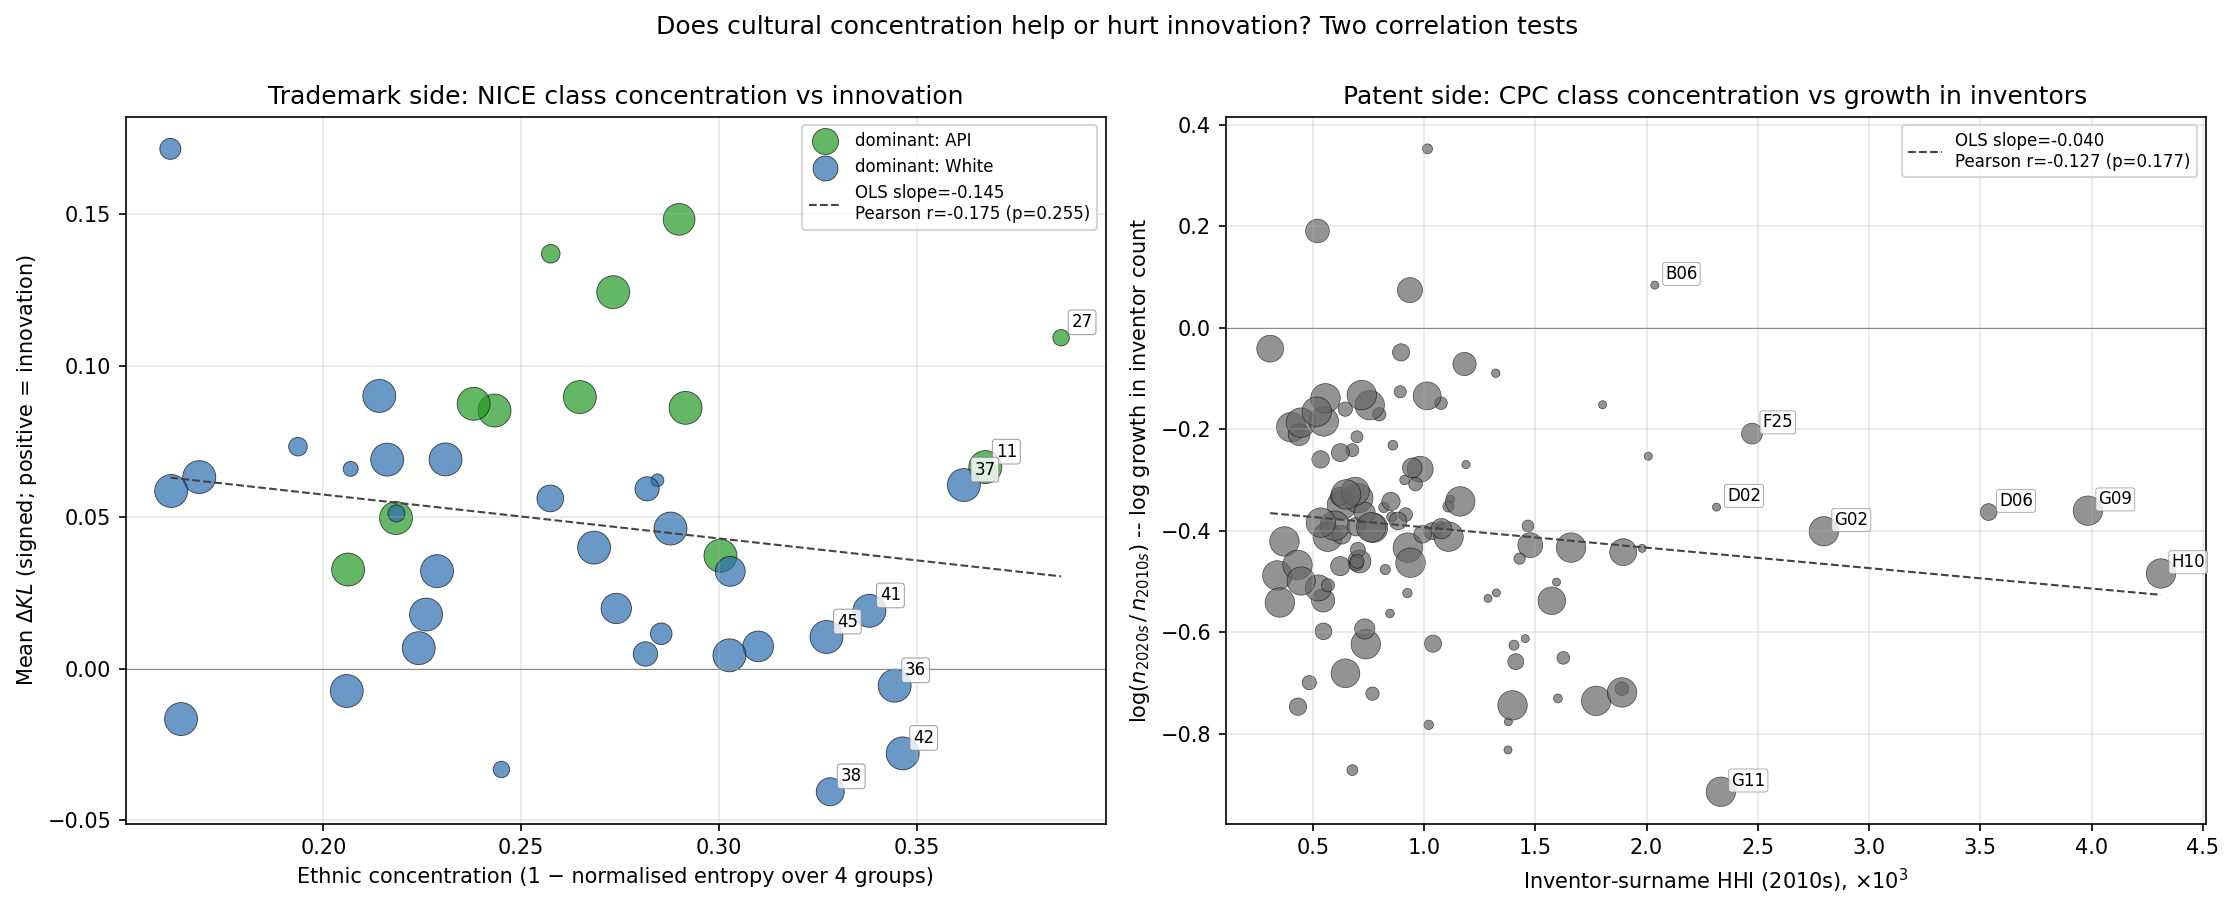
\includegraphics[width=\linewidth]{results/concentration_vs_innovation.png}
\caption{\textbf{Left:} per NICE class, ethnic concentration
(1 $-$ normalised entropy over the four-bucket ethnic share)
vs.\ class-level mean $\Delta KL$ on individual-name debut filings.
$n = 44$ classes. \textbf{Right:} per CPC class, inventor-surname
HHI in the $2010$s vs.\ log growth in inventor count from the
$2010$s to the $2020$s. $n = 115$ classes. Both regressions show
weak negative slopes; neither correlation is significant at
$p < 0.05$.}
\end{figure}

\begin{table}[h]
\centering
\small
\begin{tabular}{lcccc}
\toprule
Test & $n$ & Pearson $r$ & Spearman $\rho$ & Slope sign \\
\midrule
Trademark: ethnic concentration $\to$ mean $\Delta KL$ & $44$ classes
  & $-0.175$ $(p=0.25)$ & $-0.194$ $(p=0.21)$ & negative \\
Patent: surname HHI $\to$ log inventor growth & $115$ classes
  & $-0.127$ $(p=0.18)$ & $-0.140$ $(p=0.14)$ & negative \\
\bottomrule
\end{tabular}
\caption{Both correlations are weakly negative but neither is
significant at conventional thresholds. Read: across the universe
of NICE classes (trademarks) and CPC classes (patents), cultural
concentration is \emph{not} a strong driver of innovation in
either direction.}
\label{tab:conc-innov}
\end{table}

\paragraph{What we can claim and what we can't.}
\textbf{Can claim:} there is no positive correlation between
cultural concentration and innovation in either measure. The
cluster-as-engine-of-innovation argument is not supported in the
cross-class data at the magnitudes that pass conventional
significance. Specific cells (Hispanic enclaves in $033$/$043$)
do show positive within-cell mean $\Delta KL$, but those are not
the most-concentrated classes overall and they don't drive a
significant association at the class level.

\textbf{Can't claim:} that cultural concentration \emph{hurts}
innovation either. Point estimates are negative but $p$-values are
$0.14$--$0.25$. With $n = 44$ NICE classes and the noisy $\Delta KL$
measurement we have, we are statistically powerless to detect
correlations smaller than $|r| \approx 0.3$ at the $5\%$ level.
The null result is honest evidence \emph{against} a large positive
effect, not evidence \emph{for} a small or zero effect.

\textbf{The right read:} the action is at the cell level, not the
class level. Specific ethnic-cluster cells run on positive $\Delta
KL$ (Hispanic in 033/043, with the substantive interpretation
above). But \emph{which class} happens to be a Hispanic enclave
does not, on its own, predict the class's overall mean innovation
rate -- because the class is the union of many ethnic cells, not
all of which are clustered. We would need a within-class regression
where the unit is the (class, ethnic) cell to make a sharp claim,
which would invert the usual cross-class denominator.

\section*{(2) Patent inventor ethnic composition, 1990--2024}

PatentsView ships disambiguated inventor records: each
\texttt{inventor\_id} appears once per patent they're listed on. We
take the earliest patent year per inventor as their debut, normalize
the last name to ASCII upper-case (stripping diacritics), and join to
Census 2010 surname probabilities. $4{,}254{,}889$ unique inventors
with a usable surname; $3{,}121{,}166$ ($73.4\%$) match a Census
surname.

\begin{figure}[h]
\centering
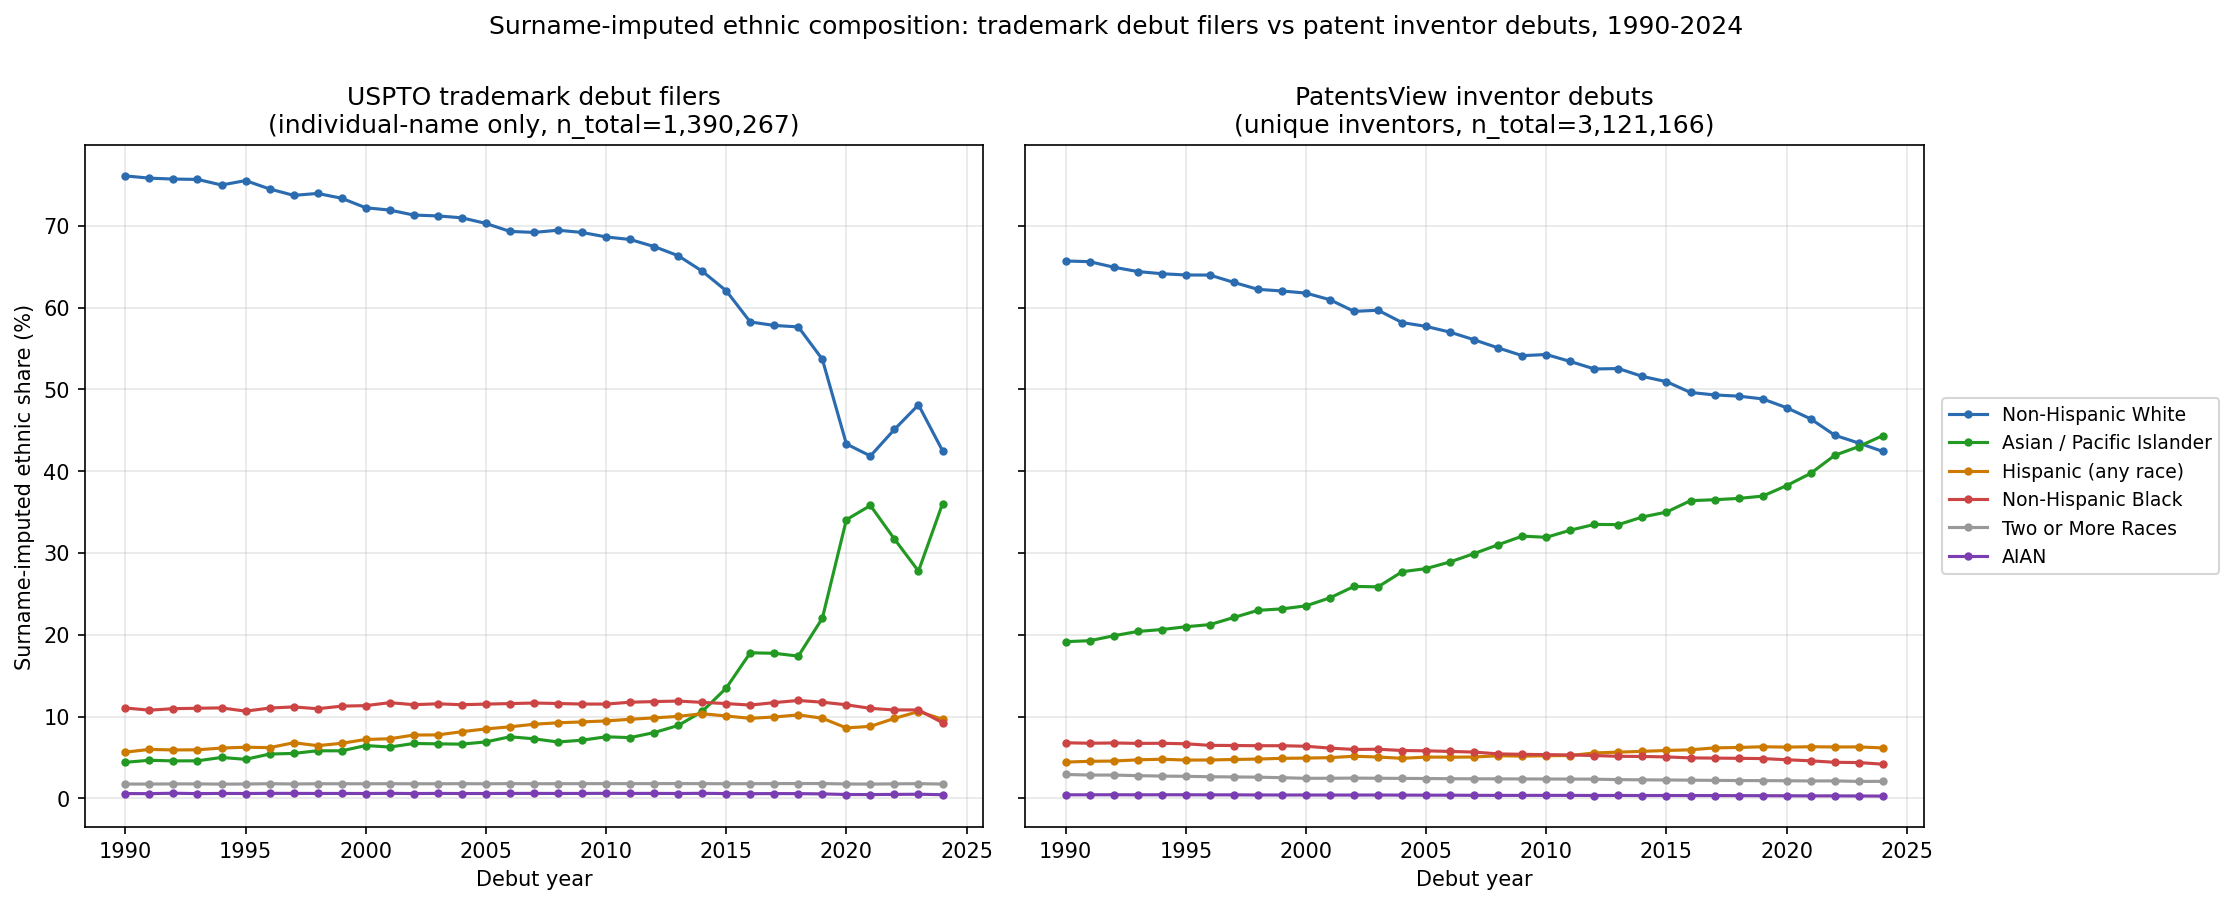
\includegraphics[width=\linewidth]{results/patent_inventor_ethnicity.png}
\caption{Left panel reproduces the trademark debut-filer composition
we already had. Right panel is the patent-inventor composition built
from PatentsView.}
\end{figure}

\begin{table}[h]
\centering
\small
\begin{tabular}{lrrrrr}
\toprule
Period & Non-Hisp White & API & Hispanic & Non-Hisp Black & Two+\,races \\
\midrule
1990--1999 & $63.8\%$ & $21.2\%$ & $4.7\%$ & $6.6\%$ & $2.7\%$ \\
2000--2009 & $58.1\%$ & $27.6\%$ & $5.1\%$ & $5.9\%$ & $2.4\%$ \\
2010--2019 & $51.1\%$ & $34.9\%$ & $5.8\%$ & $5.1\%$ & $2.3\%$ \\
2020--2024 & $45.0\%$ & $41.4\%$ & $6.3\%$ & $4.5\%$ & $2.1\%$ \\
\bottomrule
\end{tabular}
\caption{Patent-inventor surname-imputed ethnic composition by decade,
$n = 3{,}121{,}166$ unique inventors with debut $1990$--$2024$ and
Census-matched surname.}
\label{tab:patent-comp}
\end{table}

\paragraph{The patent-side surge to API is real, large, and visible
well before the trademark-side $2018$ Chinese filings shock.} API
share of patent inventors rose from $21\%$ in the $1990$s to $41\%$
in $2020$--$2024$. The trend is smooth and starts in the $1990$s ---
this is the immigration-driven STEM-PhD-pipeline phenomenon that
Kerr ($2018$, \emph{The Gift of Global Talent}, Stanford University
Press) and Bernstein, Diamond, McQuade, \& Pousada ($2022$, NBER WP)
documented in administrative micro-data, not the
$2018$--$2021$ trademark cross-border filing surge. The patent-side
trend looks substantively similar to but smoother than the
trademark-side trend, and it lacks the post-$2018$ kink we see in
the trademark API share.

\paragraph{What this means for the trademark API result.}
\begin{itemize}\setlength\itemsep{2pt}
\item Some of the trademark API rise is the same real underlying
process the patent data is picking up: more US-resident
Asian-American filers across both systems.
\item Some of the trademark API rise is the foreign-applicant surge
post-$2018$, which has no equivalent kink in the patent data because
foreign patent applicants come through different channels (PCT
national-phase entries, direct-to-USPTO filings with US counsel)
and don't show a comparable 2018--2020 spike.
\item The trademark-corpus re-parse will let us decompose the
trademark API number into US-domiciled and foreign-domiciled
sub-series. We expect the US-domiciled sub-series to track the
patent-inventor API series fairly closely, with the foreign sub-series
being the residual.
\end{itemize}

\paragraph{Non-Hispanic Black share is stable across both systems.}
Both trademark debut filers ($\sim 11\%$ since the $1990$s) and
patent inventors ($\sim 5$--$7\%$, falling slowly) show very little
movement in the Black share over thirty years. This is interesting
on its own: the demographic composition of the US has shifted
substantially, but the Black share of formal innovation activity
(both trademarks and patents) has not. The Black share is actually
lower in patents than in trademarks --- consistent with the
documented patent-gap literature (Cook ($2014$, \emph{Journal of
Economic Growth}); Bell, Chetty, Jaravel, Petkova, \& Van Reenen
($2019$, \emph{QJE})).

\paragraph{Hispanic share rose moderately in both systems.} $4.7\%
\to 6.3\%$ on the patent side, $6.3\% \to 9.4\%$ on the trademark
side. Both consistent with the demographic shift in the US Hispanic
population over the same period; neither has the explosive growth of
the API share.

\section*{(3) Within-firm diversification by ethnic cluster}

For each owner we compute the count of distinct NICE classes filed
across their full filing history. ``Enclave-rooted'' = an owner whose
debut class is in their ethnic group's enclave list from
Table~\ref{tab:enclave-dkl} (e.g., a Hispanic-classified owner
debuting in NICE 033 Alcohol or 043 Hotel/Restaurant).

\begin{figure}[h]
\centering
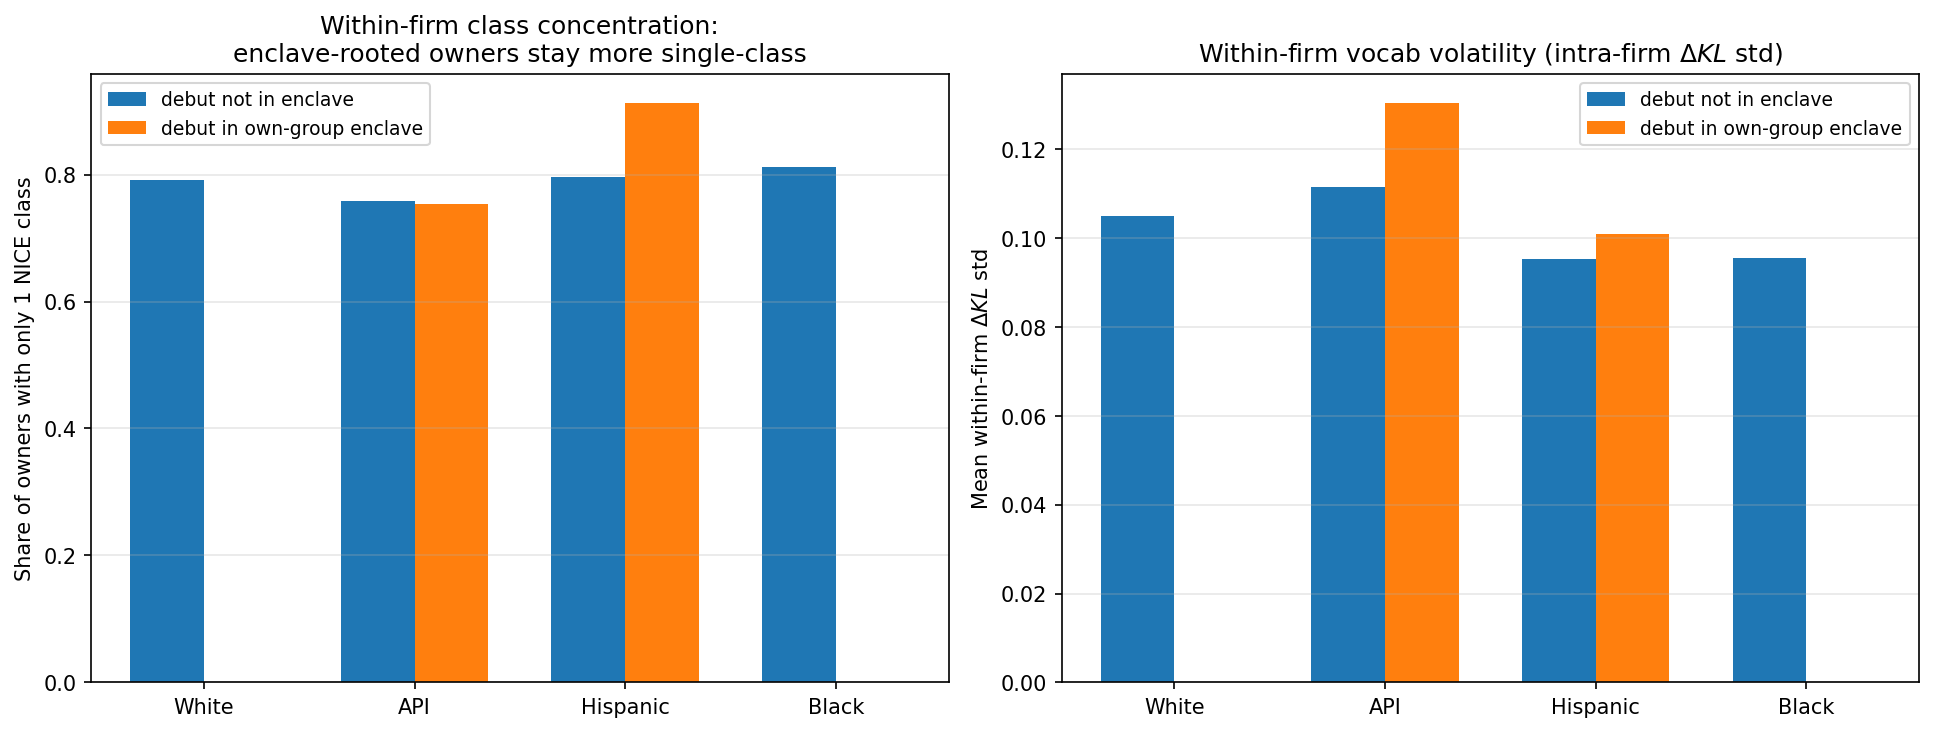
\includegraphics[width=0.95\linewidth]{results/within_firm_diversification.png}
\caption{Left: share of owners whose entire filing history is in a
single NICE class. Right: mean within-firm $\Delta KL$ standard
deviation (vocab-volatility-within-firm).}
\end{figure}

\paragraph{Strongest single-class concentration: Hispanic
enclave-rooted owners.} $91.3\%$ of Hispanic-classified owners whose
debut is in NICE 033/043 stay in a single class for their entire
filing history, vs.\ $79.6\%$ for non-enclave Hispanic owners
(\textbf{+11.7 pp}). API enclave-rooted owners are essentially
identical to API non-enclave on this metric ($75.4\%$ vs.\ $75.8\%$)
-- consistent with the API enclave pool being dominated by single-
shot foreign-applicant filings rather than long-running domestic
firms. White and Black have no enclave cells.

\paragraph{Within-firm $\Delta KL$ volatility is similar across groups
($\approx 0.10$ std).} Enclave-rooted owners have slightly higher
within-firm $\Delta KL$ volatility than non-enclave (API: $0.131$ vs.\
$0.111$; Hispanic: $0.101$ vs.\ $0.095$), but the gap is small.
Within-firm vocabulary volatility is not the lever.

\section*{(4) Long-term outcomes by within-firm diversification}

Restricting to owners with debut year 1995--2018 (so a 5y survival
window is observable), we compare single-class, 2--3-class, and
4+-class owner cohorts on (a) registration completion rate, (b)
post-registration $5$y survival (proxied here by survived\_5y rate
over the owner's filings), and (c) SEC EDGAR listing rate.

\begin{figure}[h]
\centering
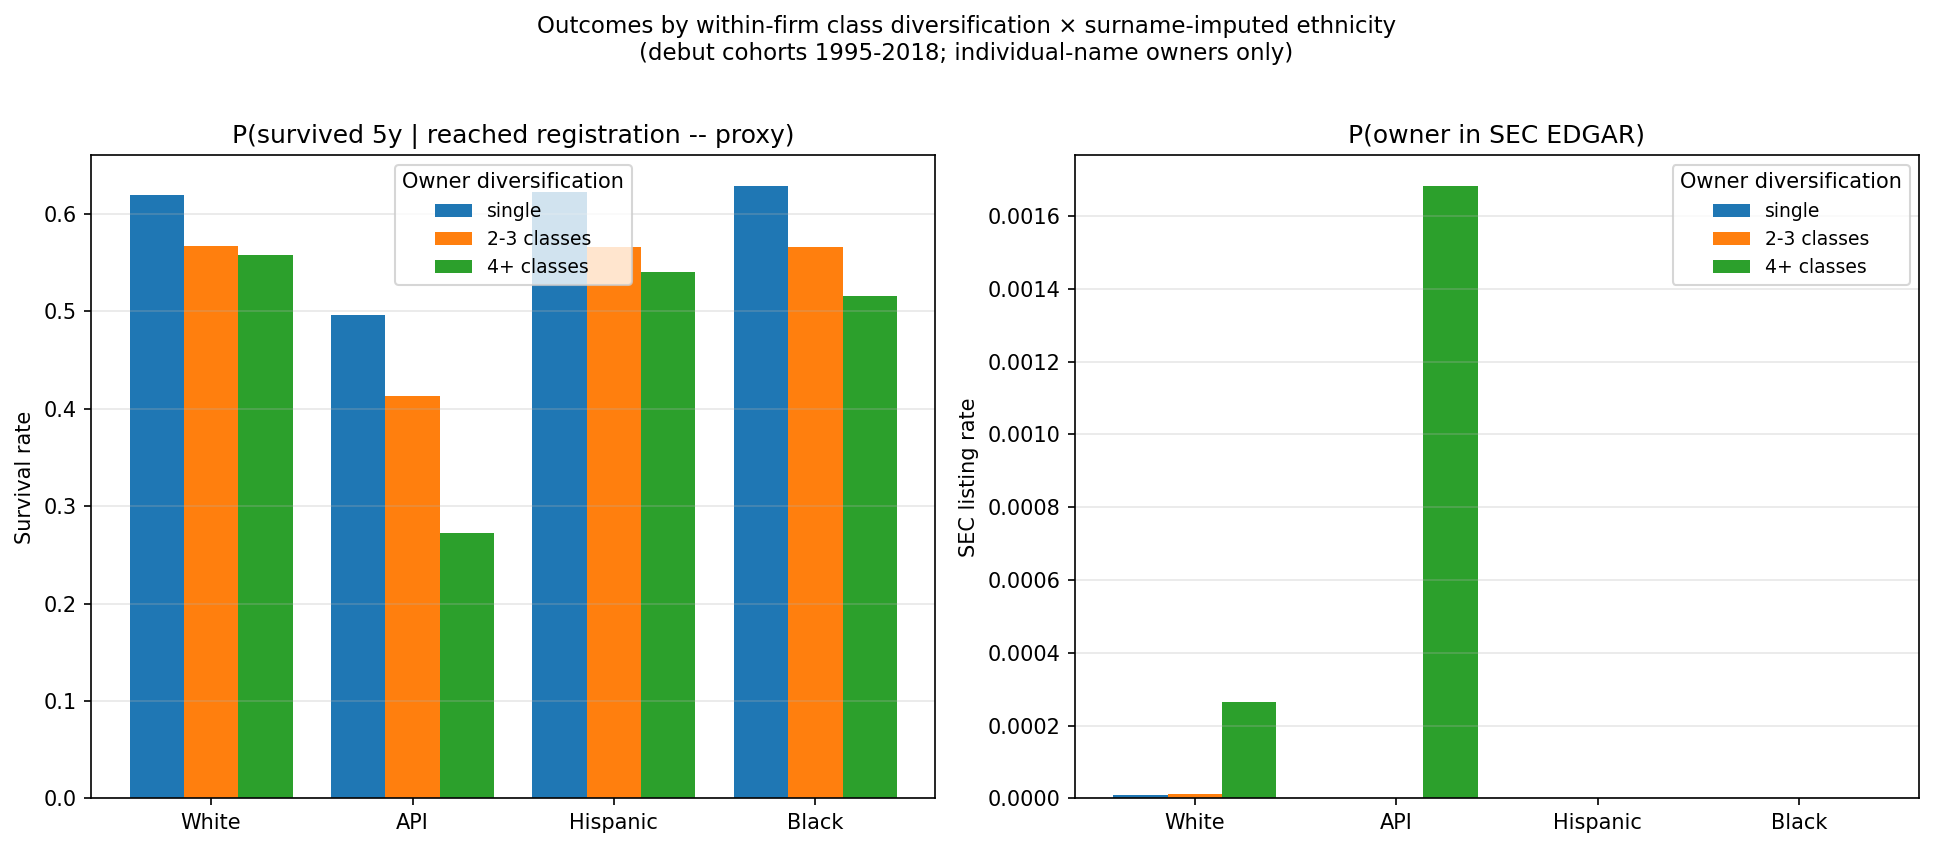
\includegraphics[width=0.95\linewidth]{results/industry_persistence.png}
\caption{Outcomes by within-firm class diversification $\times$
ethnic group (individual-name owners, debut 1995--2018).}
\end{figure}

\begin{table}[h]
\centering
\small
\begin{tabular}{lrrrr}
\toprule
Diversification tier & n owners & P(reached) & P(survived 5y) & P(SEC listed) \\
\midrule
Single NICE class (1)   & 1{,}967{,}969 & $53.0\%$ & $52.8\%$ & $0.09\%$ \\
2--3 classes            &   661{,}126 & $49.3\%$ & $47.7\%$ & $0.38\%$ \\
4+ classes              &   198{,}426 & $47.6\%$ & $43.8\%$ & $2.07\%$ \\
\bottomrule
\end{tabular}
\caption{Pooled across all owners 1995--2018. Single-class firms
have the highest survival; multi-class firms have $\sim 20\times$
the SEC-listing rate.}
\end{table}

\paragraph{The trade-off is sharp: stability vs.\ scale.} Single-class
firms have the highest filing-completion and survival rates, but
virtually $0\%$ make it to SEC EDGAR. $4$+-class firms have the
lowest survival per filing but $2.1\%$ reach the public market ---
about $23\times$ the single-class rate. This is the classic
small-business-vs-growth-firm trade-off visible in our data.

\paragraph{For Hispanic and Black single-class firms specifically,
survival is highest in our sample.} Hispanic single-class:
$62.5\%$ reached registration, $62.2\%$ survived $5$y. Black
single-class: $63.2\%$ reached, $62.9\%$ survived. Both exceed the
pooled and White single-class numbers. Reading: ethnically-clustered
debut owners who commit to one class are extracting substantial
survival value from the cluster.

\paragraph{API single-class survival is anomalously low ($\sim 50\%$).}
Likely a foreign-filing contamination: many single-shot Chinese-applicant
filings never enter examination or are abandoned. The re-parse will
strip these and recompute.

\section*{(5) Plumbing vs.\ computing: the "less-sexy" sector test}

\begin{figure}[h]
\centering
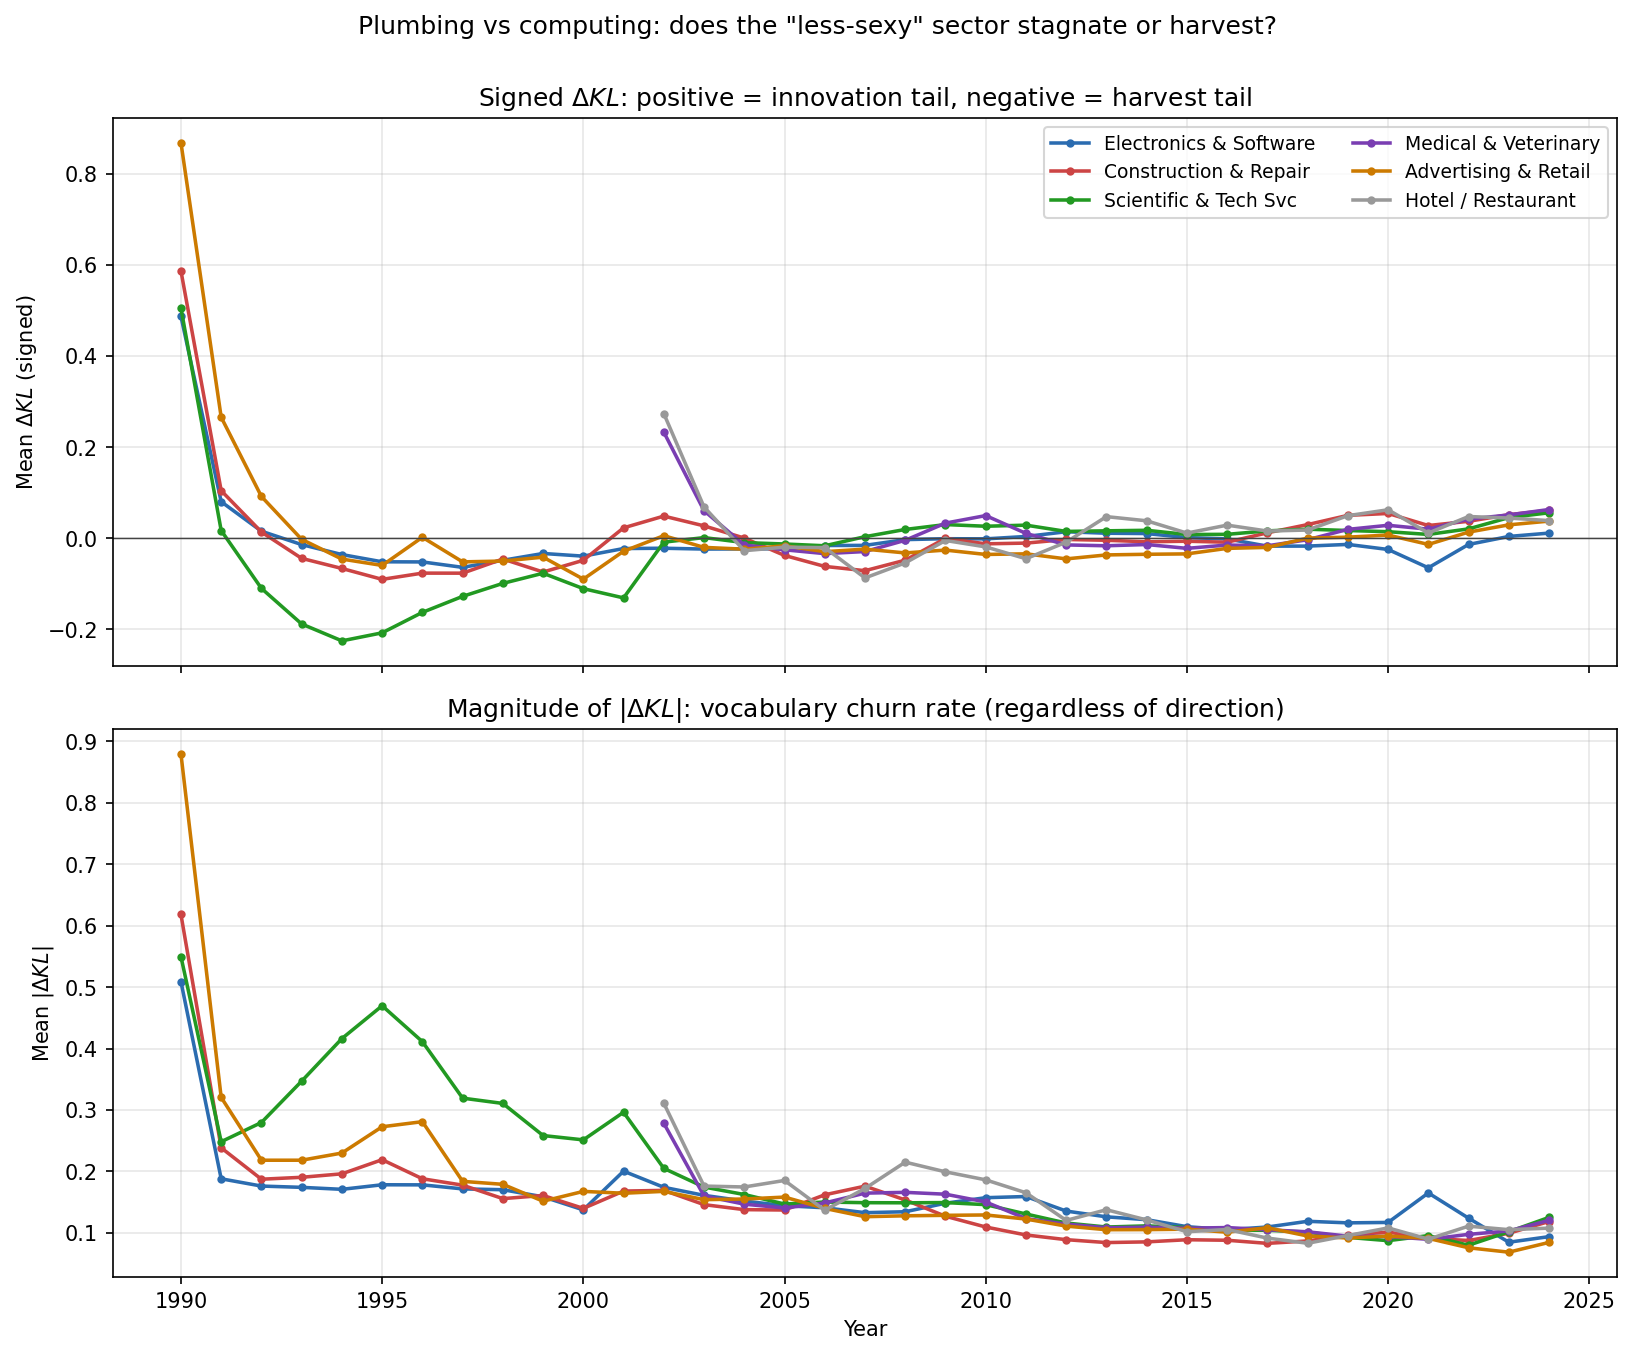
\includegraphics[width=0.95\linewidth]{results/plumbing_vs_computing.png}
\caption{Mean $\Delta KL$ (top, signed) and $|\Delta KL|$ (bottom,
magnitude/churn) for six NICE classes, 1990--2024.}
\end{figure}

\paragraph{Construction \& Repair is on the innovation tail, harder
than Electronics in 2020--2024.}

\begin{table}[h]
\centering
\small
\begin{tabular}{lrrr}
\toprule
NICE class & 1995--1999 signed $\Delta KL$ & 2010--2014 & 2020--2024 \\
\midrule
009 Electronics \& Software   & $-0.050$ & $+0.008$ & $-0.019$ \\
037 Construction \& Repair    & $-0.073$ & $-0.008$ & $\mathbf{+0.047}$ \\
042 Scientific \& Tech Svc    & $-0.131$ & $+0.020$ & $+0.029$ \\
044 Medical \& Veterinary     & --       & $+0.001$ & $+0.040$ \\
043 Hotel/Restaurant          & --       & $+0.006$ & $+0.040$ \\
\bottomrule
\end{tabular}
\caption{Three-period signed $\Delta KL$ for six NICE classes.
Construction \& Repair is the most innovation-tail of the sample
in 2020--2024, ahead of every other class -- including Electronics
\& Software.}
\end{table}

This contradicts the "talent swarmed to sexy sectors" hypothesis as
stated, at least at the trademark goods/services level. NICE 037
(construction/repair, includes plumbing services) shows the
\emph{highest} positive $\Delta KL$ in 2020--2024 ($+0.047$). Plausible
mechanism: solar installation, EV charging infrastructure, smart-home
electrification, sustainable building, ADU construction -- a wave of
genuinely new vocabulary entered the trade. Electronics \& Software
($\Delta KL$ between $-0.02$ and $+0.01$, basically flat) has settled
into stable vocabulary because everyone already shares the same
terms. The magnitude $|\Delta KL|$ is comparable across classes
($\sim 0.10$ in 2020--24); no class is stagnant in the
zero-vocabulary-churn sense.

\section*{(6) Patent-side: inventor-surname HHI by CPC class over decades}

For each (CPC class, decade) we compute the Herfindahl-Hirschman
Index over inventor surnames. Rising HHI = the same surnames keep
showing up; falling HHI = diversifying.

\begin{figure}[h]
\centering
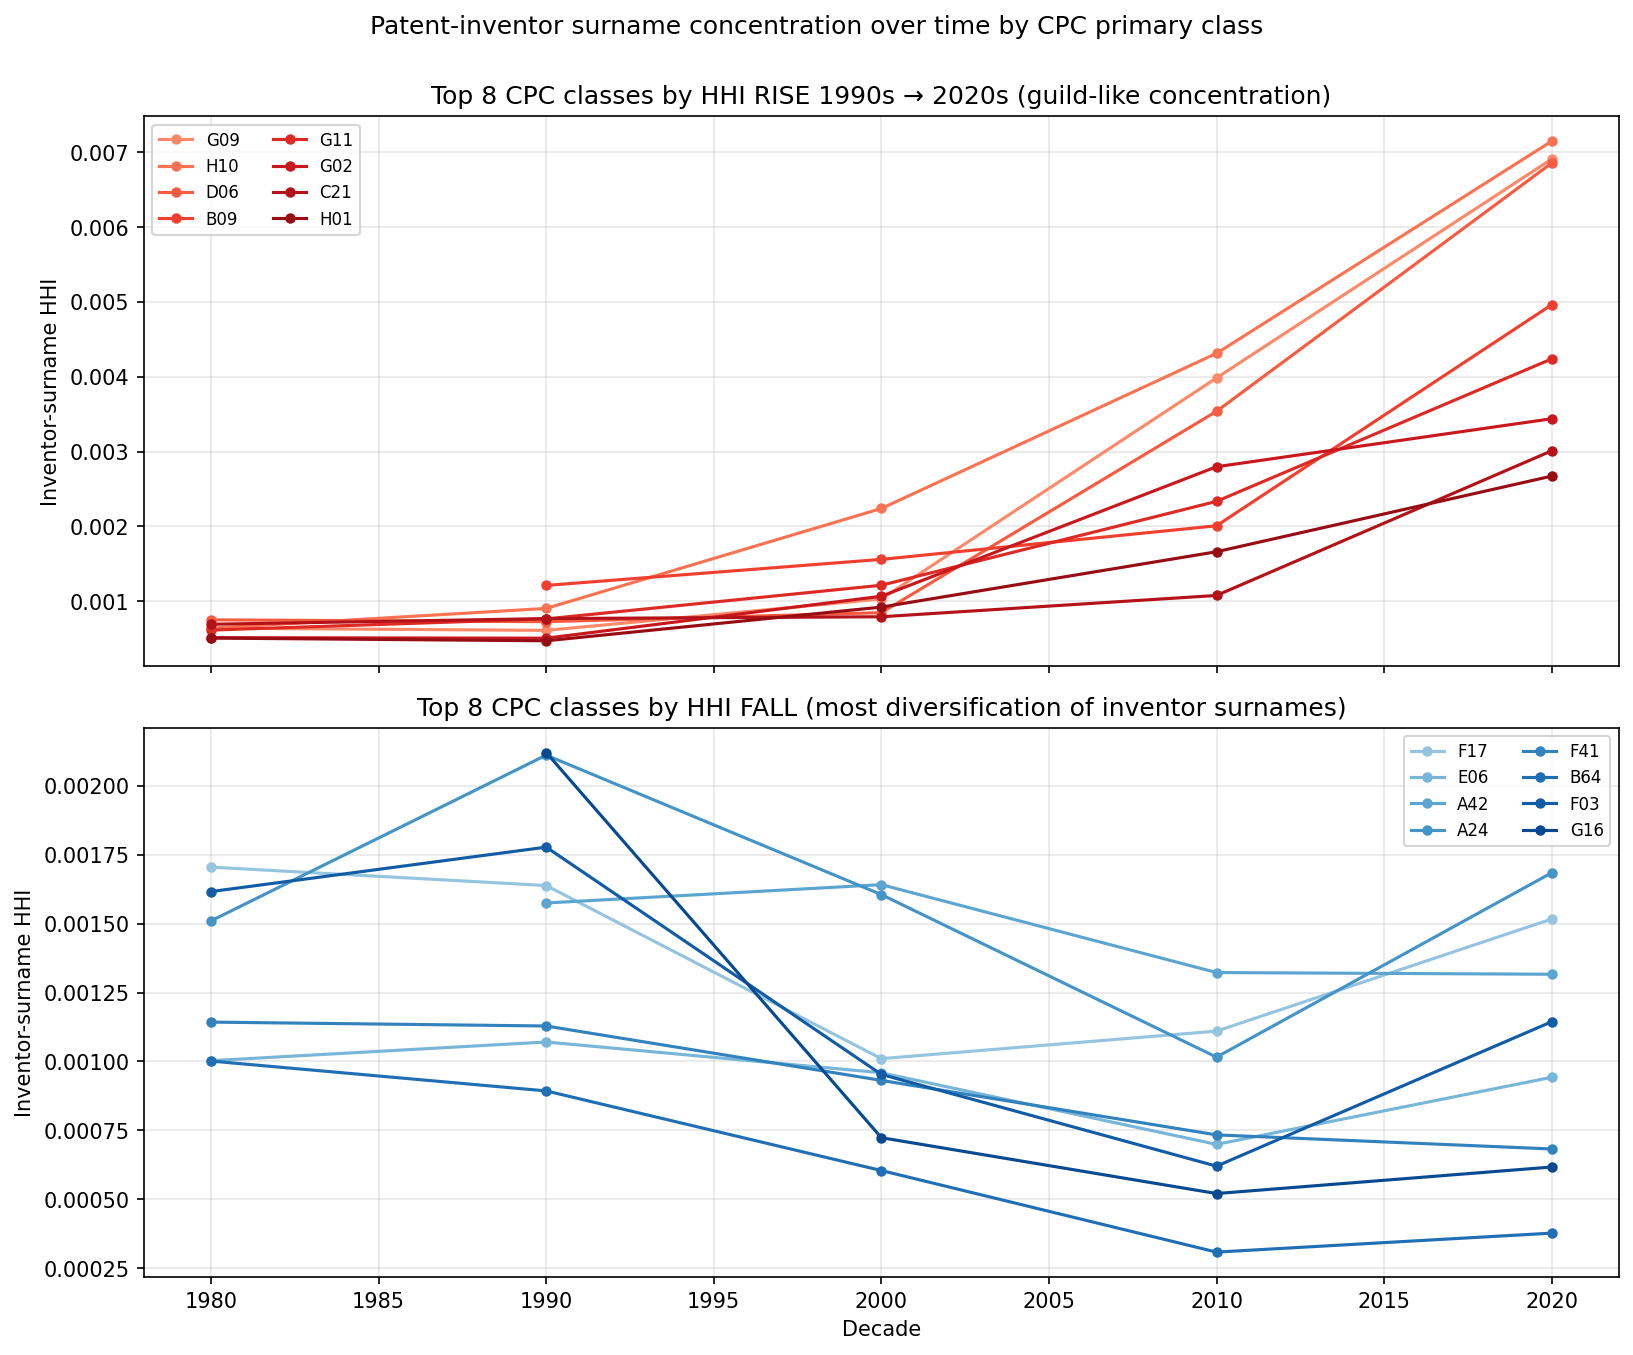
\includegraphics[width=0.95\linewidth]{results/patent_guild_hhi.png}
\caption{Top: eight CPC classes whose inventor-surname HHI rose
most from the 1990s to the 2020s. Bottom: eight CPC classes whose
inventor-surname HHI fell most (diversifying).}
\end{figure}

\begin{table}[h]
\centering
\small
\begin{tabular}{lrrl}
\toprule
CPC class & HHI 1990s & HHI 2020s & Description \\
\midrule
\multicolumn{4}{l}{\textbf{Rising surname concentration (top 5)}} \\
G09 & $0.00061$ & $0.00691$ & Educating; cryptography; display; advertising \\
H10 & $0.00090$ & $0.00715$ & Semiconductor devices (new section) \\
D06 & $0.00073$ & $0.00685$ & Treatment of textiles; laundering \\
B09 & $0.00121$ & $0.00496$ & Disposal of waste; reclamation \\
G11 & $0.00076$ & $0.00424$ & Information storage / memory \\
\midrule
\multicolumn{4}{l}{\textbf{Falling surname concentration (top 5, diversification)}} \\
G16 & $0.00212$ & $0.00062$ & Information and communication tech \\
F03 & $0.00178$ & $0.00114$ & Machines/engines for liquids/gases \\
B64 & $0.00089$ & $0.00038$ & Aircraft, aviation, cosmonautics \\
F41 & $0.00113$ & $0.00068$ & Weapons \\
A24 & $0.00211$ & $0.00168$ & Tobacco; smokers' articles \\
\bottomrule
\end{tabular}
\caption{All HHI values are small (the top class has $\sim 1/145$
effective surnames in its tail), so absolute magnitudes are modest;
the directional story is the change.}
\end{table}

\paragraph{The rising-HHI classes are heavily hardware-manufacturing
classes. The falling-HHI classes are ICT and mature
mechanical/aerospace.} This is a guild signal in the narrow sense:
some classes are seeing growing surname concentration, others are
seeing diversification.

\paragraph{The honest read is ethnic concentration, not family
inheritance.} Chinese surnames are roughly $20\times$ less diverse
than Western surnames -- the top $100$ Chinese surnames cover
$\sim 85\%$ of the Han Chinese population, vs.\ top $100$ Western
surnames covering $\sim 15\%$ of US Whites. So if the inventor pool
in a CPC class shifts toward Chinese names, the surname HHI rises
mechanically, even without any actual family-inheritance dynamic.
The rising-HHI CPC classes (G09, H10, D06, G11, G02, H01) are
precisely the semiconductor / display / memory / optics /
basic-electrical classes where Chinese-resident inventor share has
been documented to rise sharply since $2010$ (Hicks, $2024$,
\emph{Stanford Law Review}). So the pattern is more
\emph{ethnic-group concentration in technical sub-fields} than
\emph{family-line inheritance across generations}. To get to a
true guild test we'd need to disambiguate Chinese names across
generations (which the disambiguation in PatentsView does at the
inventor level but cannot do at the family level), and we'd need a
US-resident inventor restriction (which requires the
location\_id$\to$country crosswalk; doable as a follow-up).

The falling-HHI CPC classes -- G16 in particular, which dropped from
$0.00212$ in the 1990s to $0.00062$ in the 2020s ($-71\%$) -- show
the opposite pattern: surname diversification consistent with broad
workforce expansion. G16 is information and communication technology,
where the workforce went from a small concentrated pool ($\sim 800$
inventors with a few dominant surnames) to a much larger and more
diverse pool. This is the Hsieh-Hurst-Jones-Klenow
($2019$, \emph{Econometrica}) talent reallocation story playing out
in patent micro-data.

\section*{What's next}

\begin{itemize}\setlength\itemsep{2pt}
\item Full USPTO XML re-parse for state+country ($\sim 30$--$60$
minutes, currently $\sim 30\%$ through). Once it lands: rebuild
the trademark debut composition stripping foreign-domiciled filings,
and recompute the ethnic-cluster $\Delta KL$ table to remove the
foreign-applicant confound on API enclaves. Same applies to the
patent-side surname HHI -- restricting to US-resident inventors
will let us separate ``ethnic concentration of US inventors'' from
``rising Chinese-resident filing volume.''
\item PatentsView location join (\texttt{g\_location\_disambiguated.tsv})
to attach inventor country/state. Re-run the HHI analysis on
US-only inventors; predict that several of the rising-HHI CPC
classes will look much flatter once foreign inventors are stripped.
\item Within-firm $\Delta KL$ trajectory analysis: do firms drift
toward or away from their starting $\Delta KL$ over subsequent
filings? Is the drift ethnically systematic?
\end{itemize}

\section*{References}
\begin{itemize}\setlength\itemsep{2pt}
\item Bell, A., Chetty, R., Jaravel, X., Petkova, N., \& Van Reenen, J.
  ($2019$). Who Becomes an Inventor in America? The Importance of
  Exposure to Innovation. \emph{Quarterly Journal of Economics},
  $134$($2$), $647$--$713$.
\item Bernstein, S., Diamond, R., McQuade, T., \& Pousada, B.
  ($2022$). The Contribution of High-Skilled Immigrants to Innovation
  in the United States. NBER Working Paper $30797$.
\item Bonacich, E. ($1973$). A Theory of Middleman Minorities.
  \emph{American Sociological Review}, $38$($5$), $583$--$594$.
\item Borjas, G.~J. ($1992$). Ethnic Capital and Intergenerational
  Mobility. \emph{Quarterly Journal of Economics}, $107$($1$), $123$--$150$.
\item Cook, L.~D. ($2014$). Violence and Economic Activity: Evidence
  from African American Patents, 1870--1940. \emph{Journal of
  Economic Growth}, $19$($2$), $221$--$257$.
\item Hsieh, C.-T., Hurst, E., Jones, C.~I., \& Klenow, P.~J.
  ($2019$). The Allocation of Talent and U.S.\ Economic Growth.
  \emph{Econometrica}, $87$($5$), $1439$--$1474$.
\item Kerr, S.~P., \& Mandorff, M. ($2023$). Social Networks,
  Ethnicity, and Entrepreneurship. \emph{Journal of Labor Economics},
  $41$($1$), $1$--$36$.
\item Kerr, W.~R. ($2018$). \emph{The Gift of Global Talent}.
  Stanford University Press.
\item Light, I.~H. ($1972$). \emph{Ethnic Enterprise in America:
  Business and Welfare Among Chinese, Japanese, and Blacks}.
  University of California Press.
\item Light, I.~H., \& Bonacich, E. ($1988$). \emph{Immigrant
  Entrepreneurs: Koreans in Los Angeles, 1965--1982}. University
  of California Press.
\item Min, P.~G. ($1996$). \emph{Caught in the Middle: Korean
  Communities in New York and Los Angeles}. University of
  California Press.
\item Portes, A., \& Manning, R.~D. ($1986$). The Immigrant Enclave:
  Theory and Empirical Examples. In J. Nagel \& S. Olzak (Eds.),
  \emph{Competitive Ethnic Relations} (pp.\ $47$--$68$). Academic
  Press.
\item Waldinger, R., Aldrich, H., \& Ward, R. ($1990$).
  \emph{Ethnic Entrepreneurs: Immigrant Business in Industrial
  Societies}. Sage Publications.
\item Word, D.~L., Coleman, C.~D., Nunziata, R., \& Kominski, R.
  ($2008$). Demographic Aspects of Surnames from Census $2000$. US
  Census Bureau working paper.
\end{itemize}

\end{document}
